%%%%%%%%%%%%%%%%%%%%%%%%%%%%%%%%%%%%%%%%%%%%%%%%%%%%%%%%%%%%%%%%%%%%%%%%%%%%%%%%%%%%%%%
\section{Diode Clipper Circuit}
\label{subsec:diode_clipper_intro}
%%%%%%%%%%%%%%%%%%%%%%%%%%%%%%%%%%%%%%%%%%%%%%%%%%%%%%%%%%%%%%%%%%%%%%%%%%%%%%%%%%%%%%%
\begin{figure}
  \centering
  
%%%%%%%%%%%%%%%%%%%%%%%%%%%%%%%%%%%%%%%%%%%%%%%%%%%%%%%%%%%%%%%%%%%%%%%%%%%%%%%%%%%%%%%
\section{Diode Clipper Modeling}
\label{chap:diode_clipper}
%%%%%%%%%%%%%%%%%%%%%%%%%%%%%%%%%%%%%%%%%%%%%%%%%%%%%%%%%%%%%%%%%%%%%%%%%%%%%%%%%%%%%%%



%%%%%%%%%%%%%%%%%%%%%%%%%%%%%%%%%%%%%%%%%%%%%%%%%%%%%%%%%%%%%%%%%%%%%%%%%%%%%%%%%%%%%%%
\subsection{Training Data}
\label{sec:diode_clipper_training_data}
%%%%%%%%%%%%%%%%%%%%%%%%%%%%%%%%%%%%%%%%%%%%%%%%%%%%%%%%%%%%%%%%%%%%%%%%%%%%%%%%%%%%%%%

The dataset to be used for the diode clipper modeling consisted of 7 minutes and 59 seconds of guitar and bass recordings from \cite{Abesser2013} and \cite{Kehling2014} respectively. The amount of guitar recordings was roughly the same as the amount of bass recordings and their ordering was arbitrary. All recordings were single-channel and used \SI{44100}{Hz} sampling rate. 1 minute and 29 seconds (approximately 20\%) of these were used as the test set. Care was taken so that the test file begins with silence. The remaining data was split into the validation set (1 minute and 18 seconds) and the train set (5 minutes and 12 seconds) according to the 80:20 rule. The input were raw recordings and the target distorted signal was synthesized from a SPICE model of the circuit with the schematic from \Figure{fig:diode_clipper_circuit} and parameter values from \Table{tab:diode_clipper_element_parameters}. For the simulation, LTspice XVII by Analog Devices was used \cite{LTspice}. The synthesized target data sounds realistically and was previously used with success in \cite{Wright2019}.

%%%%%%%%%%%%%%%%%%%%%%%%%%%%%%%%%%%%%%%%%%%%%%%%%%%%%%%%%%%%%%%%%%%%%%%%%%%%%%%%%%%%%%%
\subsection{Training}
\label{sec:diode_clipper_training}
%%%%%%%%%%%%%%%%%%%%%%%%%%%%%%%%%%%%%%%%%%%%%%%%%%%%%%%%%%%%%%%%%%%%%%%%%%%%%%%%%%%%%%%

The training procedure was as follows. Firstly, the dataset was loaded, then the network architecture was initialized, and the training parameters were set (optimization algorithm, hyperparameters, learning rate schedule, loss function). Then the proper training was run for a fixed number of epochs. After each epoch, the validation loss was computed. Finally, after finishing the last epoch, the test set was processed and the model's output along with the final loss value were recorded.

The training set was split into half-second segments. These segments were randomly shuffled at the beginning of each epoch and split into minibatches of a predetermined size.

A single epoch consisted of processing the minibatches of segments in chunks (subsegments) of a given length. After each subsegment, the gradient of the loss with respect to the network parameters was calculated using the \ac{BPTT}. Then, the gradient step was performed using the Adam optimizer \cite{Kingma2017}, the computational graph was discarded and the next subsegment processed. After each minibatch, the learning rate scheduler performed its step (if such a scheduler was set). When an epoch ended, model parameters were stored by overwriting the previously saved ones. Additionally, the training session kept track of the model which performed best on the validation set.

The number of epochs in training was determined by manually observing the validation loss curve. If the validation loss reached a plateau below 1\% of the loss, the training was deemed successful.

%%%%%%%%%%%%%%%%%%%%%%%%%%%%%%%%%%%%%%%%%%%%%%%%%%%%%%%%%%%%%%%%%%%%%%%%%%%%%%%%%%%%%%%
\subsection{Compared Models}
\label{sec:diode_clipper_models}
%%%%%%%%%%%%%%%%%%%%%%%%%%%%%%%%%%%%%%%%%%%%%%%%%%%%%%%%%%%%%%%%%%%%%%%%%%%%%%%%%%%%%%%

For the assessment of how well ODENet can model the diode clipper, two derivative networks were chosen: $2 \times 100 \times 100 \times 1$ (ODENet100) and $2 \times 9 \times 9 \times 1$ (ODENet9), both with the \ac{ReLU} nonlinearity. The latter is the smallest derivative network that has reached validation loss smaller than 1\%. Both were trained and tested with the forward Euler scheme. Additionally, the latter was trained and tested with the implicit Adams scheme and \ac{SELU} nonlinearity.

For benchmark, the following architectures were chosen:
\begin{itemize}
    \item \ac{STN} $2 \times 4 \times 4 \times 4 \times 1$ with $\tanh$ nonlinearity and biases enabled only in the second layer from \cite{Parker2019}, 
    \item \ac{RINN} with \ac{RK}4 integration parameters (\ac{RINN}4) using a bilinear block with 6 units in each fully connected layer (BB6) from \cite{Ouala2019}, and 
    \item \ac{LSTM} with 8 hidden units and a $8 \times 1$ output \ac{MLP} (mapping the hidden states to an output sample) from \cite{Wright2019} (\ac{LSTM}8).
\end{itemize}

All of the architectures were trained on audio data at \SI{44100}{Hz} sampling rate.

Each model is listed with its number of parameters,
% TODO: computational complexity in processing (ops/sample, GFLOPS), 
hyperparameter values during training, training time (in epochs and hours), and teacher forcing curriculum in \Table{tab:diode_clipper_models_data}. The curriculum descriptions mean the following: "never" does not use teacher forcing, "always" provides true output for each minibatch, "bernoulli" uses scheduled sampling, where the probability of using teacher forcing decreases with each epoch. 
\begin{table}[]
    \caption{Compared network architectures for diode clipper modeling}
    \resizebox{\textwidth}{!}{%
\begin{tabular}{@{}l c c c c c c @{}}
\toprule
\textbf{Model} & \textbf{LSTM8} & \textbf{\makecell{STN\\3x4\\tanh}} & \textbf{\makecell{ODENet100\\(FE)\\ReLU}} & \textbf{\makecell{ODENet9\\(FE)\\ReLU}} & \textbf{\makecell{ODENet9\\(IA)\\SELU}} & \textbf{\makecell{RINN4\\BB6}} \\ \midrule
Number of   parameters & 361 & 48 & 10501 & 127 & 127 & 67 \\ 
Learning rate & 0.001 & 0.001 & 0.001 & 0.001 & 0.001 & 0.001 \\ 
Learning rate schedule & none & none & \makecell{one-cycle\\LR 0.02} & \makecell{one-cycle\\LR 0.02} & \makecell{cyclical\\LR 0.01} & \makecell{one-cycle\\LR 0.02} \\ 
Epochs in training & 200 & 340 & 300 & 300 & 600 & 600 \\ 
Hours in training & 1 & 49 & 8 & 10 & 75 & 24 \\ 
Teacher forcing & never & bernoulli & always & always & always & never \\ 
Minibatch size & 40 & 256 & 256 & 256 & 256 & 512 \\ \bottomrule
\end{tabular}%
}

    \label{tab:diode_clipper_models_data}
\end{table}

Each of these models was tested on previously unseen data at \SI{44100}{Hz} (same as training data), \SI{22050}{Hz}, \SI{48000}{Hz}, and \SI{192000}{Hz} sampling rates. The goal in using various sampling rates at test time was to analyze the presence of aliasing in the output. Test loss $\mathcal{E}(y, \hat{y})$ given by \Equation{eq:final_loss_function}, \ac{segSNR} given by \Equation{eq:seg_snr}, and \ac{ODG} described in 
% TODO: Add section including the ODG
were calculated for each model and test sampling rate.

All models were tested on a one long sequence but the implicit Adams scheme consistently diverged in this test setting. Therefore, its tests were conducted using segments of 22050 samples which were concatenated afterwards.

%%%%%%%%%%%%%%%%%%%%%%%%%%%%%%%%%%%%%%%%%%%%%%%%%%%%%%%%%%%%%%%%%%%%%%%%%%%%%%%%%%%%%%%
\subsection{Results and Discussion}
\label{sec:diode_clipper_results}
%%%%%%%%%%%%%%%%%%%%%%%%%%%%%%%%%%%%%%%%%%%%%%%%%%%%%%%%%%%%%%%%%%%%%%%%%%%%%%%%%%%%%%%

In \Table{tab:diode_clipper_results} the test results of the compared models are shown. Loss and \ac{segSNR} are rounded to two significant digits, whereas \ac{ODG} is rounded to three significant digits. The best results are given in bold (lowest loss, highest \ac{segSNR} and \ac{ODG}). The models are separately evaluated in terms of the learned model quality (test sampling rate equal to training sampling rate) and performance at sampling rates different from the training sampling rate. 

% ODENet @ 22kHz test sampling rate goes into self oscillations

\begin{table}[]
    \caption{Test results of the diode clipper models.}
    \newcommand{\modelNameCellWidth}{1.8cm}
    \resizebox{\textwidth}{!}       & 0.91\%            & 0.1\% & 0.38\% & 0.12\% & 0.19\% \\ \cmidrule(l){3-9} 
        \multicolumn{1}{|l|}{} &  & \makecell{segSNR\\$\times 10^{-4}$}  & 2.7              & 2.7          & 2.5          & 2.5 & \textbf{3} & 2.7 \\ \cmidrule(l){3-9} 
        \multicolumn{1}{|l|}{} &  & ODG     & -1.7                 & -2.1             & -1.64 & \textbf{-1.54}    & -2 & -1.57 \\ \cmidrule(l){2-9} 
        \multicolumn{1}{|l|}{} & \multirow{3}{*}{22050} & 
                                    Loss    & \textbf{0.088\%}       & 230\%          & 530\% & 29\% & 65\% & 0.48\% \\ \cmidrule(l){3-9} 
        \multicolumn{1}{|l|}{} &  & \makecell{segSNR\\$\times 10^{-4}$}  & 2.5              & 2          & -1.6 & 2.4 & -25 & \textbf{2.84} \\ \cmidrule(l){3-9} 
        \multicolumn{1}{|l|}{} &  & ODG     & -3.9                 & -3.9             & -3.9 & -3.9 & -3.9 & -3.9 \\ \cmidrule(l){2-9} 
        \multicolumn{1}{|l|}{} & \multirow{3}{*}{48000} & 
                                    Loss    & \textbf{0.065\%}       & 0.37\%            & 0.092\% & 0.32\% & 0.085\% & 0.16\% \\ \cmidrule(l){3-9} 
        \multicolumn{1}{|l|}{} &  & \makecell{segSNR\\$\times 10^{-4}$}  & 2.5              & 2.7          & 2.7 & 2.6 & \textbf{3.1} & 2.9 \\ \cmidrule(l){3-9} 
        \multicolumn{1}{|l|}{} &  & ODG     & -1.42                 & -1.64             & -1.47 & \textbf{-1.41} & -1.67 & -1.43 \\ \cmidrule(l){2-9} 
        \multicolumn{1}{|l|}{} & \multirow{3}{*}{192000} & 
                                    Loss    & 0.58\%                & 0.35\%            & \textbf{0.062\%} & 0.2\% & 0.075\% & 0.55\% \\ \cmidrule(l){3-9} 
        \multicolumn{1}{|l|}{} &  & \makecell{segSNR\\$\times 10^{-4}$}  & -0.4             & 2.6          & 2.8 & 2.7 & \textbf{3.2} & 2.9 \\ \cmidrule(l){3-9} 
        \multicolumn{1}{|l|}{} &  & ODG     & -3.56                 & -1.55             & -3.58 & \textbf{-1.46} & -1.54 & -3.54 \\ \bottomrule
    \end{tabular}%
    }
    \label{tab:diode_clipper_results}
\end{table}

%%%%%%%%%%%%%%%%%%%%%%%%%%%%%%%%%%%%%%%%%%%%%%%%%%%%%%%%%%%%%%%%%%%%%%%%%%%%%%%%%%%%%%%
\subsubsection{Model Quality}
%%%%%%%%%%%%%%%%%%%%%%%%%%%%%%%%%%%%%%%%%%%%%%%%%%%%%%%%%%%%%%%%%%%%%%%%%%%%%%%%%%%%%%%

The model quality in terms of the loss function is very good for all compared architectures. In casual listening, only the \ac{RINN}4 model sounds differently from the target (despite the low test loss value). Their \ac{segSNR} values are comparatively low with the ODENet9(IA) receiving slightly better results than others. Its forward Euler version, ODENet9(FE), has the highest \ac{ODG}. Somewhat surprisingly, the smaller ODENet models outperformed the larger one in terms of \ac{segSNR} and \ac{ODG}. This could be explained by the fact that limiting the model capacity has a regularizing effect \cite{Goodfellow-et-al-2016}.

Results better or comparable to the established \ac{LSTM} and \ac{STN} architectures prove that ODENet is suitable for diode clipper modeling. Although the diode clipper is quite simple to learn, the results provide a proof of concept that ODENet, extended to incorporate an input signal into its processing, could be used for \ac{VA} modeling.

%%%%%%%%%%%%%%%%%%%%%%%%%%%%%%%%%%%%%%%%%%%%%%%%%%%%%%%%%%%%%%%%%%%%%%%%%%%%%%%%%%%%%%%
\subsubsection{Behavior at Unseen Sampling Rates}
%%%%%%%%%%%%%%%%%%%%%%%%%%%%%%%%%%%%%%%%%%%%%%%%%%%%%%%%%%%%%%%%%%%%%%%%%%%%%%%%%%%%%%%

For \SI{22050}{Hz} test sampling rate (half of the training sampling rate), the lowest loss value was obtained for \ac{LSTM} with 8 hidden units. The second best result (\ac{RINN}4) was already an order of magnitude worse, with the remaining models obtaining over a hundred times worse results. The highest \ac{segSNR} was achieved by \ac{RINN}4. \ac{LSTM} sounds best and quite accurately in casual listening. However, the output of \ac{STN} as well as all ODENet models contain high amount of digital distortion. Moreover, ODENet100(FE) and ODENet9(IA) fall into self-oscillations, i.e., contain a constant high-frequency component even when input signal is very quiet. Although the digital distortion sounds unpleasantly, it is a sign that the networks learned the true derivative (or residual in the case of \ac{STN}) contained in the data. The derivative networks probably output a correct value but given a larger time step without any additional tuning, the produced sound contains components beyond the Nyquist frequency, which causes aliasing in the output sound. Contrary to the casually perceived quality of \ac{LSTM}, all produced outputs received equally low \ac{ODG}. 

For \SI{48000}{Hz} test sampling rate, again \ac{LSTM} received the best loss value, yet all models had test loss value smaller than 1\%. In terms of \ac{segSNR} and \ac{ODG}, smaller ODENet models again took the lead as for \SI{44100}{Hz} sampling rate. In casual listening, there is not much difference between the model outputs.

For \SI{192000}{Hz} test sampling rate, the advantage of the ODENet becomes clear with the larger model having the lowest loss value and smaller models outperforming all the other ones with respect to \ac{segSNR} and \ac{ODG}. As could be expected, architectures that take sampling rate into account during processing (\ac{STN}, ODENet) obtained lower loss value and significantly higher \ac{ODG}. The output of \ac{LSTM} sounds significantly distorted in comparison to other architectures, suggesting that this architecture may not be the most optimal option for processing at sampling rates higher than in training. 

All in all, ODENet architectures outperformed other models in terms of \ac{segSNR} and \ac{ODG} for all test sampling rates higher than training sampling rate. What is more, they continued to have loss value smaller than 1\% for those sampling rates. It was possible even for the simplest numerical scheme, i.e., the forward Euler. Therefore, ODENet is suitable for training at one sampling rate and processing at a higher one.

There was no clear advantage of the implicit solver over the explicit one. On the contrary, the implicit solver took over twice the time to process the same amount of data as the explicit solver did, as indicated in \Table{tab:diode_clipper_models_data}.For the diode clipper model, it does not seem beneficial to increase the derivative network's capacity beyond the necessary minimum (here: 9 hidden units). 

%%%%%%%%%%%%%%%%%%%%%%%%%%%%%%%%%%%%%%%%%%%%%%%%%%%%%%%%%%%%%%%%%%%%%%%%%%%%%%%%%%%%%%%
\subsubsection{Convergence Speed}
%%%%%%%%%%%%%%%%%%%%%%%%%%%%%%%%%%%%%%%%%%%%%%%%%%%%%%%%%%%%%%%%%%%%%%%%%%%%%%%%%%%%%%%

\begin{figure}
    \centering
    \begin{tikzpicture}
    \begin{axis}[
        no markers,
        every axis plot/.append style={ultra thick},
        xmin = 0,
        xmax = 200,
        grid,
        xlabel = Epoch,
        ylabel = Validation Loss,
    ]
        \addplot[smooth,mark=none,color=blue, dashed] table [x=Step, y=Value, col sep=comma] {figures/tikz/diode_clipper_validation_curves/run-forward_euler_July16_13-14-04_axel_ODENet2Hidden9-tag-Loss_validation.csv};
        \addplot[smooth,mark=none,color=red] table [x=Step, y=Value, col sep=comma] {figures/tikz/diode_clipper_validation_curves/run-lstm_June30_13-57-49_axel-tag-Loss_validation.csv};
        \legend{ODENet9(FE), LSTM8};
    \end{axis}
\end{tikzpicture}

    \caption{Convergence curves of the diode clipper models.}
    \label{fig:diode_clipper_validation_curves}
\end{figure}

Looking at how validation loss of ODENet and LSTM changes during training, as shown in \Figure{fig:diode_clipper_validation_curves}, one can observe that the former takes much more epochs to get below 1\% than the latter. This may be explained by the nature of the \ac{LSTM} architecture, where the constant-error carousel ensures that error gets propagated even for very long time lags \cite{Hochreiter1997}. Slow convergence can be seen as a disadvantage of the ODENet framework, slowing down the derivative network architecture exploration or hyperparameter search. Increasing the learning rate of the ODENet, for example using one-cycle learning rate schedule, has proven itself beneficial but must be used with care; if the learning rate is too large, ODENet diverges.

%%%%%%%%%%%%%%%%%%%%%%%%%%%%%%%%%%%%%%%%%%%%%%%%%%%%%%%%%%%%%%%%%%%%%%%%%%%%%%%%%%%%%%%
\subsubsection{Comparison to Numerical Solvers}
%%%%%%%%%%%%%%%%%%%%%%%%%%%%%%%%%%%%%%%%%%%%%%%%%%%%%%%%%%%%%%%%%%%%%%%%%%%%%%%%%%%%%%%



  \caption{Diode clipper circuit.}
  \label{fig:diode_clipper_circuit}
\end{figure}

The first-order diode clipper is a circuit frequently used to achieve signal distortion, e.g., in guitar amplifiers. Its schematic is shown in \Figure{fig:diode_clipper_circuit}. It can be regarded as consisting of two parts: an RC lowpass filter and a diode limiter.

Voltages and currents in this section are dependent on time, i.e., $V = V(t), I= I(t)$. For readability, this dependence is not stated explicitly in the equations.

%%%%%%%%%%%%%%%%%%%%%%%%%%%%%%%%%%%%%%%%%%%%%%%%%%%%%%%%%%%%%%%%%%%%%%%%%%%%%%%%%%%%%%%
\subsection{RC Lowpass Filter}
%%%%%%%%%%%%%%%%%%%%%%%%%%%%%%%%%%%%%%%%%%%%%%%%%%%%%%%%%%%%%%%%%%%%%%%%%%%%%%%%%%%%%%%

\begin{figure}
  \centering
  \begin{tikzpicture}
%--------start graphics code --------
% \draw[step=0.5,very thin, black!20] (-1,-0.5) grid (6,2.5);
\path (0,0) coordinate (ref_gnd);
\draw
  (ref_gnd)++(0,2) node[ocirc] {}
  node[xshift=-2mm,yshift=4mm] {$V_{in}$}
  to [R=\(R\)] ++(2,0) node[circ] {}
  to ++(1,0)  node[ocirc] {}
  node[yshift=4mm] {$V_{out}$}
  ++(-1,0)
  to [C=\(C\)] ++(0,-2)
  node[ground] {};
%--------end graphics code ----------
\end{tikzpicture}

  \caption{RC lowpass filter.}
  \label{fig:rc_lowpass}
\end{figure}

The first part of the diode clipper circuit is an RC lowpass filter. An RC lowpass filter is shown in \Figure{fig:rc_lowpass}. Given that the input voltage $V_\text{in}$ is a sine wave at frequency $f$, the input-output voltage relation is governed by the following equation
\begin{equation}
  V_\text{out} = \frac{X_C}{\sqrt{R^2 + X_C^2}} V_\text{in},
  \label{eq:rc_circuit}
\end{equation}
where $V_\text{out}$ is the output voltage, $X_C=\frac{1}{2\pi f C}$ is the capacitive reactance of the capacitor in the circuit, $C$ is its capacitance, and $R$ is the resistor's resistance.

The capacitor impedes low frequencies more; the lower the frequency, the higher the capacitive reactance. More capacitive reactance means larger voltage drop on the capacitor. Thus, assuming a constant magnitude across all frequencies of the input voltage, the output voltage is higher for low frequencies. Therefore, the circuit behaves like a lowpass filter.

Considering an arbitrary input waveform, we may derive a differential equation that describes the circuit \cite{Horowitz2015}. The current $I$ through the capacitor is proportional to the rate of change of the voltage across it

\begin{equation}
  I = C \frac{\mathrm{d}V_\text{out}}{\mathrm{d} t}.
  \label{eq:current_through_capacitor}
\end{equation}

The current flowing through the resistor can be calculated using the Ohm's law as a ratio of the voltage drop across the resistor to its resistance

\begin{equation}
  I = \frac{V_\text{in} - V_\text{out}}{R}.
  \label{eq:current_through_resistor}
\end{equation}

Because the same current flows through the resistor and the capacitor we can equate the right-hand sides of \Equation{eq:current_through_capacitor} and \Equation{eq:current_through_resistor}. After dividing by $C$, we obtain the final form of the \ac{ODE} describing the RC circuit

\begin{equation}
  \frac{\mathrm{d}V_\text{out}}{\mathrm{d} t} = \frac{V_\text{in} - V_\text{out}}{RC}.
\end{equation}



%%%%%%%%%%%%%%%%%%%%%%%%%%%%%%%%%%%%%%%%%%%%%%%%%%%%%%%%%%%%%%%%%%%%%%%%%%%%%%%%%%%%%%%
\subsection{Diode Limiter}
%%%%%%%%%%%%%%%%%%%%%%%%%%%%%%%%%%%%%%%%%%%%%%%%%%%%%%%%%%%%%%%%%%%%%%%%%%%%%%%%%%%%%%%
\begin{figure}
  \centering
  \input{figures/tikz/diode_limiter.tex}
  \caption{Diode limiter circuit.}
  \label{fig:diode_limiter}
\end{figure}

The second part of the diode clipper is the diode limiter also called a \emph{diode clamp} \cite{Malvino2016}. Its circuit is shown in \Figure{fig:diode_limiter}. It consists of two inversely polarized diodes and a resistor. This circuit could be further divided into a \emph{positive clipper} (by removing the diode on the left) and a \emph{negative clipper} (by removing the diode on the right). These names refer to which part of the input \ac{AC} signal (the positive or the negative) is removed at the output.

If the diodes were ideal, i.e., they would behave as an open for voltages across smaller than 0 and as a short for voltages across larger than 0, $V_\text{out}$ would always be 0. However, to a second approximation, the diodes cause a voltage drop of \SI{0.7}{V} when conducting. Thus, the voltage cannot exceed the \SIrange{-0.7}{0.7}{V} range, being clamped when attempting to do so. The positive clipper guards the upper limit and the negative clipper guards the lower limit. The effect of passing an \ac{AC} signal through the diode limiter is shown in \Figure{fig:diode_limiter_signal}.

The analytical derivation of the differential equation governing the diode limiter circuit is more challenging than that of the first-order lowpass. Yeh et al. \cite{Yeh2007} present a small-signal interpretation of the diode limiter circuit.

\begin{figure}
  \centering
  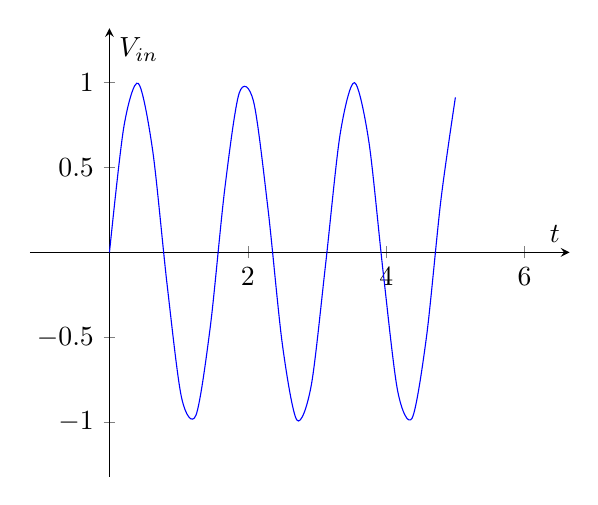
\begin{tikzpicture}
    \begin{axis}[
        domain=0:5,
        axis lines = middle,
        xmin = -0.5,
        xmax = 6,
        ymin = -1.1,
        ymax = 1.1,
        xlabel = $t$,
        ylabel = $V_{in}$,
        enlargelimits = true,
    ]
        \addplot[smooth,mark=none,color=blue] {sin(4*deg(x))};
    \end{axis}
\end{tikzpicture}
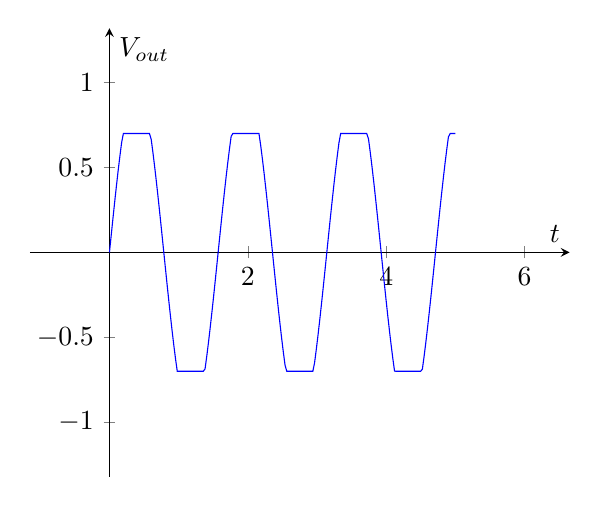
\begin{tikzpicture}
    \begin{axis}[
        domain=0:5,
        axis lines = middle,
        xmin = -0.5,
        xmax = 6,
        ymin = -1.1,
        ymax = 1.1,
        xlabel = $t$,
        ylabel = $V_{out}$,
        enlargelimits = true,
        y filter/.expression={y > 0.7 ? 0.7 : (y < -0.7 ? -0.7 : y)},
    ]
        \addplot[samples=200,mark=none,color=blue] {sin(4*deg(x))};
    \end{axis}
\end{tikzpicture}

  \caption{Impact of the diode limiter on the input sinusoidal voltage. Values that exceed the \SIrange{-0.7}{0.7}{V} range are clamped and the signal is distorted.}
  \label{fig:diode_limiter_signal}
\end{figure}


%%%%%%%%%%%%%%%%%%%%%%%%%%%%%%%%%%%%%%%%%%%%%%%%%%%%%%%%%%%%%%%%%%%%%%%%%%%%%%%%%%%%%%%
\subsection{First-Order Diode Clipper}
%%%%%%%%%%%%%%%%%%%%%%%%%%%%%%%%%%%%%%%%%%%%%%%%%%%%%%%%%%%%%%%%%%%%%%%%%%%%%%%%%%%%%%%
Combining the RC lowpass filter (\Figure{fig:rc_lowpass}) and the diode limiter (\Figure{fig:diode_limiter}) yields the first-order diode clipper (\Figure{fig:diode_clipper_circuit}). It is called "first-order" because only a single capacitor is used \cite{Parker2019}. If the input voltage is within the limiter's operational range, the circuit acts as a lowpass filter. If the voltage exceeds this range, it is clipped at the output and distortion is introduced.

The first-order diode clipper can be described by a nonlinear \ac{ODE} \cite{Yeh2007}
\begin{equation}
  \frac{\mathrm{d} V_\text{out}}{\mathrm{d}t} = \frac{V_\text{in} - V_\text{out}}{RC} - 2 \frac{I_\text{s}}{C} \sinh \left(\frac{V_\text{out}}{V_\text{t}}\right),
  \label{eq:diode_clipper_equation}
\end{equation}
where $V_\text{in}$ is the input voltage (typically on the order of volts), $V_\text{out}$ is the output voltage, $t$ denotes time, $R$ is the serial resistance, $C$ is the parallel capacity, $I_\text{s}$ is the reverse saturation current, and $V_\text{t}$ is the thermal voltage. The last two are parameters of the diodes that can be measured \cite{Yeh2007}.

The parameter values of discrete elements used in the experiments were taken from \cite{Yeh2008}. They are summarized in \Table{tab:diode_clipper_element_parameters}.

\begin{table}
  \centering
  \begin{tabular}{c c}
    \toprule
    \textbf{Parameter} & \textbf{Value} \\
    \midrule
    $R$ & \SI{2.2}{k\ohm} \\
    $C$ & \SI{10}{nF} \\
    $I_\text{s}$ & \SI{2.52}{nA} \\
    $V_\text{t}$ & \SI{45.3}{mV} \\
    \hline
  \end{tabular}
  \caption{Parameter values of the discrete elements used in the diode clipper circuit. Source:~\cite{Yeh2008}.}
  \label{tab:diode_clipper_element_parameters}
\end{table}

%%%%%%%%%%%%%%%%%%%%%%%%%%%%%%%%%%%%%%%%%%%%%%%%%%%%%%%%%%%%%%%%%%%%%%%%%%%%%%%%%%%%%%%
\subsection{Relation to Other Work}
%%%%%%%%%%%%%%%%%%%%%%%%%%%%%%%%%%%%%%%%%%%%%%%%%%%%%%%%%%%%%%%%%%%%%%%%%%%%%%%%%%%%%%%

The first-order diode clipper is a system particularly interesting in the context of ODENet, because it is governed by a known \ac{ODE} \cite{Yeh2007,Yeh2008}. Additionally, it was already modeled using a \ac{ResNet}-like architecture in \cite{Parker2019}. Thus, learning to imitate the diode clipper allowed the validation of ODENet and comparison to 
\begin{itemize}
    \item an \ac{LSTM}-based architecture from \cite{Wrightetal2020},
    \item a \ac{ResNet}-like architecture from \cite{Parker2019}, and
    \item a numerical solution using the \ac{ODE} from \cite{Yeh2007,Yeh2008}.
\end{itemize}
